\documentclass[a4paper, 10pt, conference]{IEEEtran}

\IEEEoverridecommandlockouts

\usepackage[utf8]{inputenc}
\usepackage[T1]{fontenc}
\usepackage[colorlinks=true,linkcolor=black,anchorcolor=black,citecolor=black,filecolor=black,menucolor=black,runcolor=black,urlcolor=black]{hyperref}
\usepackage{graphicx}
\usepackage[ngerman]{babel}
\usepackage[style=ieee]{biblatex}

\addbibresource{references.bib}

\graphicspath{ {./images/} }

\begin{document}

\title{\LARGE \bf
SGDb: Semantic Video Game Database
}

\author{
\IEEEauthorblockN{Anastasia Chernysheva} \IEEEauthorblockA{\textit{a.chernysheva@oth-aw.de}}\and
\IEEEauthorblockN{Jakob Götz} \IEEEauthorblockA{\textit{j.goetz@oth-aw.de}}\and
\IEEEauthorblockN{Ardian Imeraj} \IEEEauthorblockA{\textit{a.imeraj@oth-aw.de}}\and
\IEEEauthorblockN{Patrice Korinth} \IEEEauthorblockA{\textit{p.korinth@oth-aw.de}}\and
\IEEEauthorblockN{Philipp Stangl} \IEEEauthorblockA{\textit{p.stangl1@oth-aw.de}}\and
}

\maketitle
\thispagestyle{empty}
\pagestyle{empty}


\begin{abstract}
    Wir beschäftigen uns mit der Speicherung und Suche vernetzter Informationen von Videospielen.
    Dazu stellen wir \textit{SGDb} vor -- eine webbasierte Anwendung mit einer Graphen-basierten Suche von Videospielen.
\end{abstract}


\section{Einleitung}\label{sec:einleitung}

Das erste Videospiel \textit{Tennis for Two} aus dem Jahr 1958 ebnete den Weg für die Spieleindustrie. Über Jahrzehnten hinaus kamen immer mehr verschiedene Spiele auf den Markt, die sich in ihrer Art und Weise unterscheiden. Mit den heutigen Videospielen ist es möglich, sich mit Spielern aus der ganzen Welt zu messen oder gemeinsam zu spielen. Aus den unzählig veröffentlichen Videospielen ist eine breite Palette an Genres entstanden. Dabei wird in der Spieleindustrie grob in sechs Kategorien unterschieden, hierbei zählen die Strategie- und Action-Spiele zu den beliebtesten Genres~\cite{statistica}. Zu den anderen vier Kategorien zählen die Rollen-, Abenteuer-, Simulationen- und sonstige Spiele. Jedes dieser Kategorien besitzt weitere Unterkategorien, die sich in ihrer Art und Weise unterscheiden.\\

Um einen Überblick zu erhalten, wie die Spiele zusammenhängen, präsentieren wir hier eine plattformunabhängige Anwendung, welche die Spiele in einem Graphen darstellt. In Abschnitt~\ref{sec:verwandte_arbeiten} des Konzeptpapiers werden bereits bestehende Anwendungen vorgestellt, die sich mit der Kategorisierung von Spielen und Darstellung von Graphen beschäftigen.
In Abschnitt~\ref{sec:anforderungen} werden die Anforderungen in Form von User Stories beschrieben. Zum Schluss wird auf die geplanten Technologien bei der Umsetzung des Projekts eingegangen, welche in Abschnitt~\ref{sec:methoden} beschrieben werden.


\section{Verwandte Arbeiten}\label{sec:verwandte_arbeiten}

Die \textit{Internet Video Games Database} (IGDB)~\cite{igdb} gibt einen Eindruck, was ein Nutzer von einer Videospieldatenbank erwarten kann. IGDB umfasst derzeit 217.233 Spiele, eine Suchfunktion, die Möglichkeit Videospiele zu entdecken (z.B.\ kürzlich veröffentlichte Videospiele), und eine Entwickler-API. Über die API können Entwickler auf die Videospieldaten mittels Protokolle wie REST oder ProtoBuf zugreifen.

Wie die Visualisierung eines Graphen möglicherweise aussehen kann, demonstriert die Anwendung Obsidian. Diese erstellt aus von Nutzern kreierten Markdown Dateien eine Graphenoberfläche. Über Verlinkungen zwischen den Markdown Dateien wächst der Graph an. Der Nutzer kann den Graph filtern oder gewisse Teile daraus hervorheben (vgl. Abbildung~\ref{fig:obsidian}).

\begin{figure}[thpb]
    \centering
    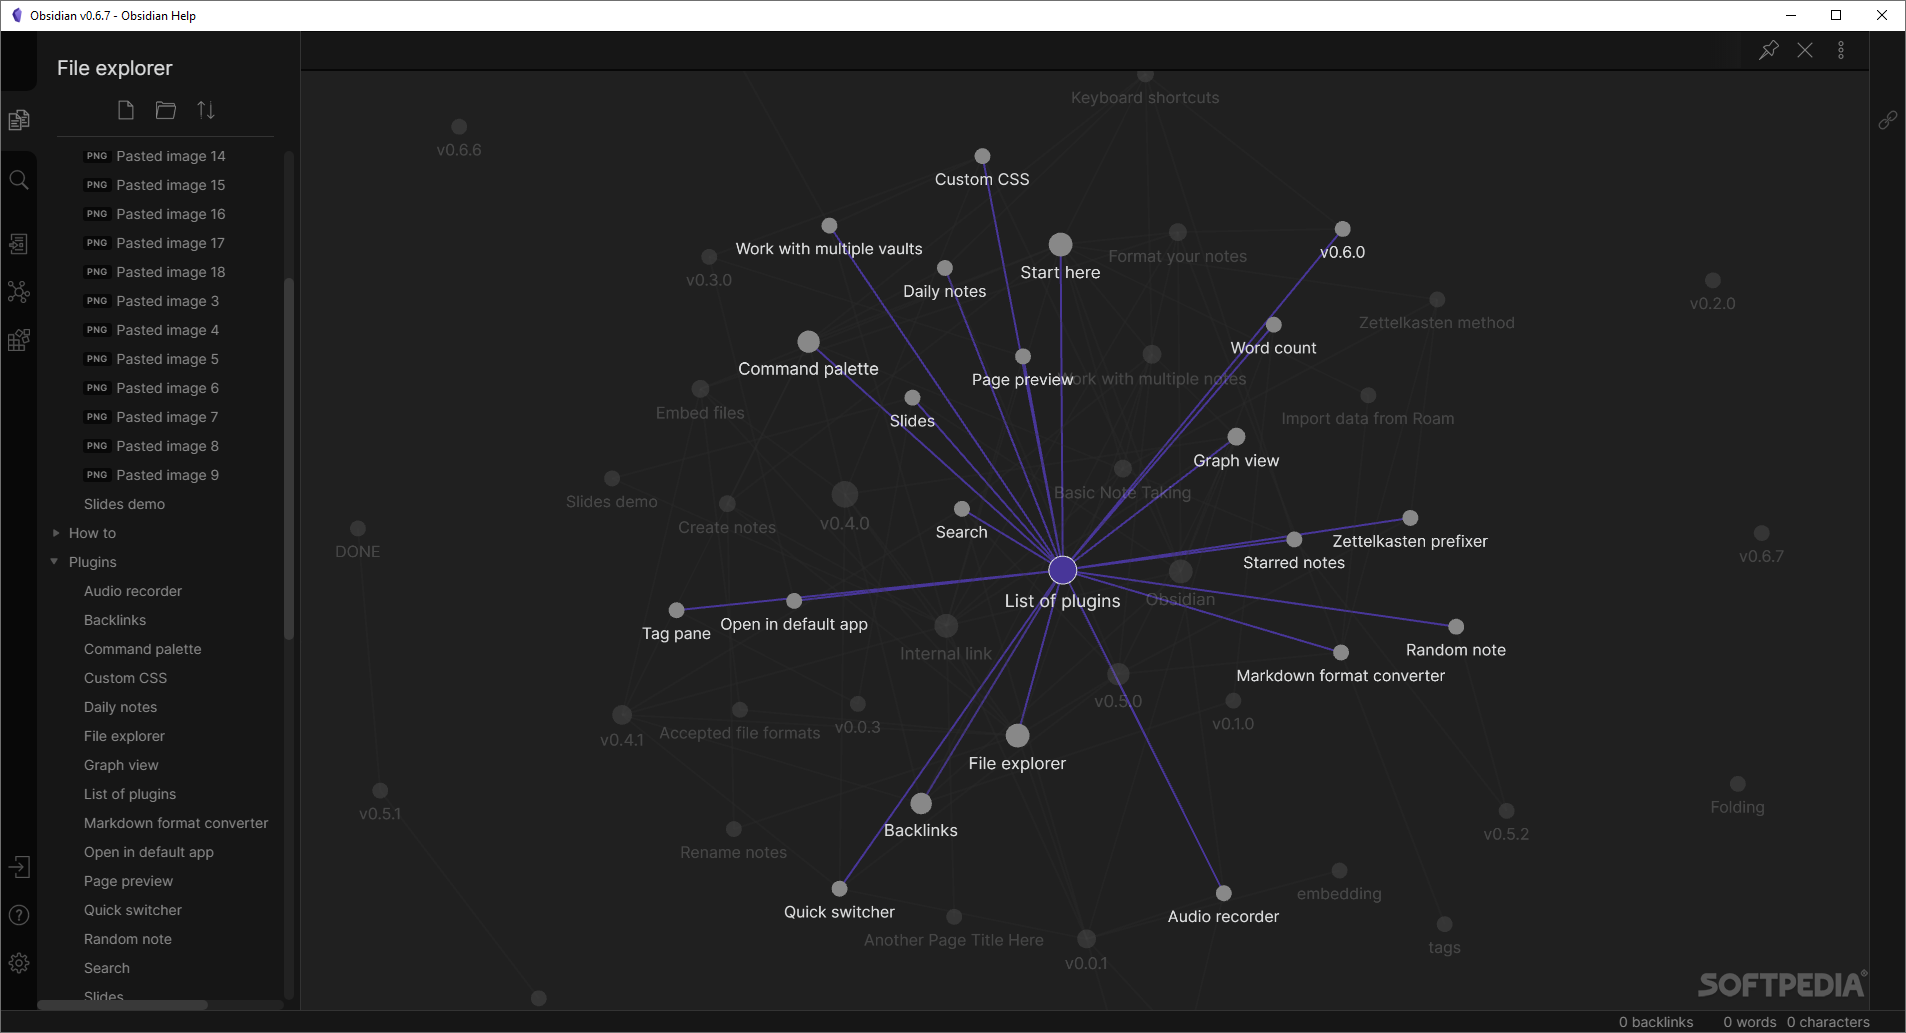
\includegraphics[scale=0.17]{obsidian}
    \caption{Obsidian Benutzeroberfläche~\cite{obsidian}}
    \label{fig:obsidian}
\end{figure}


\section{Anforderungen}\label{sec:anforderungen}

In der Anforderungsanalyse wurden zwei primäre Ziele identifiziert, die es umzusetzen gilt: (1) Die Überführung von relationalen Videospieldaten aus IGDB in eine semantische Graphdatenbank, und (2) die Möglichkeit zur Suche von Videospielen per Graph oder Texteingabe.


\subsection{Suche per Graph}

Als Benutzer möchte ich in eine Graphenoberfläche, welche visuell Verbindungen zu anderen Spielen aufzeigt. Somit kann ich direkt ähnliche Spiele, welche mir ebenfalls gefallen könnten, sehen. Akzeptanzkriterien sind:
\begin{itemize}
	\item Auf der Startseite ist ein Graph vorhanden, der alle in der Datenbank vorhandenen Videospiele und deren Beziehungen zueinander anzeigt.
    \item Schwebt man mit der Maus über einen Knoten öffnet sich ein Informationsfeld, indem angezeigt wird:
    \begin{itemize}
      \item Titel des Videospiels
      \item Genre
      \item Bewertung
    \end{itemize}
    \item Schwebt man mit der Maus über einen Knoten werden alle verbundenen Knotenpunkte und Kanten im Graphen hervorgehoben.
\end{itemize}


\subsection{Suche per Texteingabe}

Als Benutzer möchte ich ein Videospiel per Texteingabe suchen können, da sich ein spezielles Spiel bei einem Graphen mit vielen Knoten und Kanten ggf. nur schlecht finden lässt. Akzeptanzkriterien sind:
\begin{itemize}
    \item Ein Eingabefeld für die textuelle Suche ist vorhanden.
    \item Ist die Suche erfolgreich, werden relevante Knotenpunkte und Kanten im Graphen hervorgehoben.
    \item Ist die Suche fehlerhaft oder liefert kein Ergebnis, wird der Benutzer darüber benachrichtigt.
\end{itemize}


\subsection{Detailseite für Videospiel}

Als Benutzer möchte ich eine Detailseite zu einem jeweiligen Videospiel, damit ich ohne die Anwendung zu verlassen die wichtigsten Informationen zu einem Spiel einsehen kann. Akzeptanzkriterien sind:
\begin{itemize}
    \item Die Detailseite öffnet sich per Klick auf einen Knoten im Graphen.
    \item Details zum Videospiel die angezeigt werden:
    \begin{itemize}
    	\item Titel
    	\item Erscheinungsdatum
    	\item Beschreibung
    	\item Bewertung
    	\item Genre
    	\item (Optional) Internetpräsenz (z.B. offizielle Website)
    \end{itemize}
    \item (Optional) Anzeige des Videospiel-Covers.
\end{itemize}


\subsection{Filteroption}\label{subsec:filter}

Als Benutzer möchte ich mit einer Filteroption Knoten und somit Spiele im Graphen visuell hervorheben. Dadurch kann auch in einem großen Graphen der Nutzer eine Gruppe von Spielen finden. Akzeptanzkriterien sind:
\begin{itemize}
	\item Eine Schaltfläche für die Filteroption ist vorhanden.
    \item Filtermöglichkeiten sind: 
    \begin{itemize}
      \item Genre
      \item Plattform
      \item Hersteller
      \item Erscheinungsjahr
    \end{itemize}
    \item Nur das Filterergebnis soll im Graphen sichtbar sein.
    \item Wird der Filter aufgehoben sollen alle entfernten Knoten wieder angezeigt werden.
\end{itemize}


\subsection{Testabdeckung}

Als Entwickler möchte ich eine ausreichende Testabdeckung, damit Fehler frühzeitig erkannt werden.
Akzeptanzkriterien sind:
\begin{itemize}
    \item Die Abdeckungsrate liegt bei mindestens 50\%.
    \item Sowohl Frontend- als auch Backend-Code wird mit geeignetem Testwerkzeug getestet.
\end{itemize}


\subsection{(Optional) Cloud-Kompatibilität}

Als Entwickler möchte ich eine Cloud-kompatible Anwendung für eine Bereitstellung der Anwendung.  Akzeptanzkriterien sind:
\begin{itemize}
    \item Für jede Komponente der Anwendung ist ein Dockerfile erstellt und lauffähig.
    \item Mit Docker Compose ist eine YAML-Datei vorhanden, um mit einem einzigen Befehl alle Container zu starten und zu beenden.
    \item (Optional) Die Anwendung ist bei einem Cloud-Anbieter (z.B. Amazon Web Services) bereitgestellt und erreichbar.
\end{itemize}


\section{Methoden}\label{sec:methoden}

Ziel bei der Entwicklung und bei der späteren Verwendung ist eine plattformunabhängige Anwendung, die eine Schnittstelle für die \textit{Linked Open Data Cloud} als auch der Bedienoberfläche der Anwendung bereitstellt. Daraus ergeben sich folgende technische Schlüsselbausteine:

Für die Repräsentation der semantischen Daten im Frontend wird das Framework Svelte verwendet. Die Daten werden voraussichtlich in einer Ontotext GraphDB Instanz persistiert. Im Backend wird FastAPI für eine REST-Schnittstelle und RDFLib zum arbeiten mit RDF verwendet. Die Kommunikation zwischen Frontend und Backend wird über die RESTful-API abgewickelt. Die einzelnen Komponenten der Anwendung (Frontend, Backend und Datenbank) werden mittels Docker \textit{containerisiert}.


\printbibliography

\end{document}
